% COMP 4900E - Real-Time Operating Systems
% Final Report: RTOS-Based Railway Block Control System
% Compile: pdflatex FinalReport.tex (twice for TOC)

\documentclass[11pt,a4paper]{article}

\usepackage[utf8]{inputenc}
\usepackage[T1]{fontenc}
\usepackage{lmodern}
\usepackage{geometry}
\usepackage{graphicx}
\usepackage{booktabs}
\usepackage{hyperref}
\usepackage{enumitem}
\usepackage{amsmath}
\usepackage{siunitx}
\usepackage{tikz}
\usetikzlibrary{arrows.meta,positioning}

\geometry{margin=1in}
\hypersetup{
  colorlinks=true,
  linkcolor=blue,
  citecolor=blue,
  urlcolor=blue
}

\title{RTOS-Based Railway Block Control System:\\
Centralized Resource Reservation and Deadlock Management on QNX Neutrino}
\author{%
Peien Liu, Kina Zhan, Samarth Arora, Jonathan Chan\\[0.5em]
\textit{Carleton University}\\
\textit{COMP 4900E --- Real-Time Operating Systems}
}
\date{April 2026}

\begin{document}
\maketitle

\begin{abstract}
This report describes the design and implementation of a deterministic railway \emph{interlocking} simulation on QNX Neutrino. A centralized \texttt{DeadlockManager} process arbitrates exclusive access to track blocks using synchronous message passing, while \texttt{TrainController} orchestrates per-train client processes that request and release blocks according to a simple route model. The system combines a mutex-protected resource table, periodic physics ticks driven by a monotonic timer, a depth-first-search-based cycle detector on a train--track resource graph, and recovery actions that break artificial deadlocks while flagging unresolvable head-on conflicts. The work realizes themes from our project proposal---O-Train-inspired single-track contention, real-time scheduling concerns, and ties to railway deadlock literature---in executable C code with reproducible example scenarios.
\end{abstract}

\tableofcontents
\newpage

% ---------------------------------------------------------------------------
\section{Introduction}

\subsection{Scope}
The deliverable is a two-process QNX application written in C: a server (\texttt{DeadlockManager}) that loads a track graph from configuration, grants at most one train per track block, advances simulated train motion on a fixed tick, and detects or mitigates circular wait; and a controller (\texttt{TrainController}) that loads trains from configuration, spawns one process per train, and exchanges IPC with the manager. Shared message layouts and limits live in the \texttt{Common} headers.

\subsection{Motivation}
Railway control must prevent both collisions and indefinite stand-offs on shared infrastructure. Single-track segments and junctions create competition for blocks; without a single authority enforcing non-conflicting routes, trains can enter circular wait (deadlock) or opposing movements on one line (head-on risk). Our proposal framed this as an RTOS problem: deterministic scheduling, priority-aware message delivery, and explicit resource ownership maps align with how safety-critical controllers are structured~\cite{dal2021tick,zhao2015review,putra2023survey}.

\subsection{Accomplishments}
We implemented:
\begin{itemize}[noitemsep]
  \item A QNX \texttt{name\_attach} / \texttt{name\_open} service architecture with \texttt{MsgSend}/\texttt{MsgReceive} request--reply IPC.
  \item Exclusive per-track allocation (\emph{block model}) with grant/deny/release logging.
  \item A \SI{10}{\milli\second} monotonic timer pulse that drives position updates and periodic deadlock checks.
  \item DFS-based cycle detection on a resource allocation graph and rollback-style recovery for certain cycles.
  \item Detection of opposing head-on requests on adjacent blocks, treated as unresolvable by automatic recovery.
  \item Example track and train configurations under \texttt{examples/} demonstrating basic routing, a resolvable cycle, and stress cases.
\end{itemize}

\subsection{Overview}
Figure~\ref{fig:arch} summarizes the architecture. Trains connect to the manager by name; the manager may call back into \texttt{TrainController} to fetch authoritative train metadata. Each train also exposes a per-train channel for tick-synchronized position updates.

\begin{figure}[htbp]
  \centering
  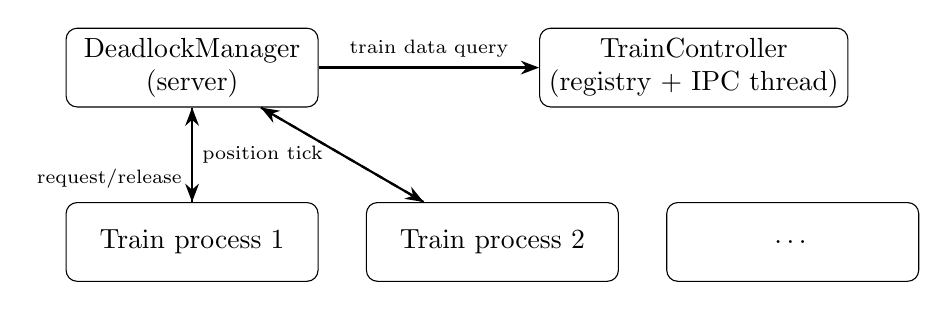
\begin{tikzpicture}[
    proc/.style={draw, rounded corners, minimum width=3.2cm, minimum height=1cm, align=center},
    arrow/.style={-{Stealth}, thick}
  ]
    \node[proc] (dm) {DeadlockManager\\(server)};
    \node[proc, right=2.8cm of dm] (tc) {TrainController\\(registry + IPC thread)};
    \node[proc, below=1.2cm of dm] (t1) {Train process 1};
    \node[proc, right=0.6cm of t1] (t2) {Train process 2};
    \node[proc, right=0.6cm of t2] (td) {\dots};
    \draw[arrow] (t1) -- node[left, font=\scriptsize, near start] {request/release} (dm);
    \draw[arrow] (t2) -- (dm);
    \draw[arrow] (dm) -- node[above, font=\scriptsize] {train data query} (tc);
    \draw[arrow, dashed] (dm) -- node[right, font=\scriptsize] {position tick} (t1);
    \draw[arrow, dashed] (dm) -- (t2);
  \end{tikzpicture}
  \caption{High-level processes and IPC. Solid lines: blocking message passing; dashed: manager-initiated position updates per train channel.}
  \label{fig:arch}
\end{figure}

\subsection{Contributions}
Team members aligned with the proposal's division of labor: interlocking and deadlock logic and validation; physics and predictive elements (occupancy, timing, stuck detection); routing and simulation of topology; RTOS IPC, scheduling-related integration, and communication paths. This report reflects the \emph{integrated} codebase rather than individual file authorship.

% ---------------------------------------------------------------------------
\section{Background}

\subsection{Railway interlocking and blocks}
An \emph{interlocking} ensures that switches, signals, and track circuits are consistent with authorized movement. We abstract the network as undirected connectivity between track identifiers; each \emph{block} may host at most one train at a time in our model, matching the proposal's emphasis on centralized reservation.

\subsection{Deadlock in single-track networks}
Deadlocks arise when trains hold blocks while waiting for others' blocks, forming a cycle in the wait-for graph. The proposal cited the ``Tick Formulation'' line of work for deadlock detection and avoidance in rail traffic control~\cite{dal2021tick}. Our implementation uses a constructed bipartite-style directed graph (trains and tracks as nodes) and DFS to detect cycles.

\subsection{QNX Neutrino primitives}
We rely on QNX's native messaging (synchronous, priority inheritance options where applicable), named channels (\texttt{name\_attach}), and timer pulses tied to the manager's channel for periodic work. \texttt{pthread} mutexes guard shared track state across message handlers and the timer path.

% ---------------------------------------------------------------------------
\section{System Design and Implementation}

\subsection{Shared protocol (\texttt{Common})}
\texttt{ipc\_protocol.h} defines message types: track request and release, acknowledgements and denials, train data query/reply, position updates, and a reroute suggestion hook for recovery analysis. \texttt{train\_data\_t} carries identity, current track, destination, route buffer, nominal speed, length, front and rear positions, entry time, and current speed. \texttt{track\_data\_t} stores occupancy pointers, nominal length, direction metadata, and up to four endpoint ids for adjacency. \texttt{system\_constants.h} fixes \texttt{TRACK\_COUNT}, \texttt{TRAIN\_COUNT}, and retry limits shared by both sides.

\subsection{DeadlockManager}
\subsubsection{Startup and configuration}
The manager requires a track configuration file path. Each non-comment line defines \texttt{track\_id}, optional length, direction, and four endpoint fields. Tracks are stored in a global array indexed by id; default block length applies when omitted.

\subsubsection{Resource manager}
\texttt{resource\_manager.c} maintains \texttt{track\_table[]}: exclusive ownership per track. \texttt{request\_track} grants if the block is free or already held by the same train; \texttt{release\_track} clears ownership and removes the train from the track's train list. This enforces the safety invariant of at most one train per block in the allocation layer.

\subsubsection{Physics engine}
\texttt{physics\_engine.c} implements constant-speed motion along a one-dimensional block: front and rear positions update from elapsed monotonic time. Helpers compute collision overlap on intervals, occupancy percentage, and track updates during ticks. The manager calls \texttt{update\_track\_data} on each tick for tracks that hold trains.

\subsubsection{Timer and tick loop}
A monotonic timer fires every \SI{10}{\milli\second} (\texttt{TICK\_INTERVAL\_NS}), delivering a pulse to the manager's channel. On each tick, the manager updates physics, sends \texttt{MSG\_POSITION\_UPDATE} to each active train's channel (\texttt{Train\#}), and every ten ticks runs \texttt{check\_deadlock\_and\_recover}.

\subsubsection{Deadlock detection and recovery}
\texttt{deadlock\_detector.c} builds a resource graph from \texttt{train\_request\_state\_t}: each train records the block it holds and the block it is waiting for. Edges connect trains to held tracks and tracks to waiting trains. DFS detects a back-edge cycle; the first train id found in the cycle is returned.

Recovery distinguishes two cases:
\begin{itemize}[noitemsep]
  \item \textbf{Head-on adjacency:} if two trains on neighboring blocks each request the other's block, the manager logs an unresolvable head-on conflict and denies movement; no safe automatic swap exists in this policy.
  \item \textbf{Other cycles:} \texttt{resolve\_deadlock\_cycle} releases the held block of a chosen train in the cycle, zeros its position state, and forces wait speed, breaking the wait-for cycle.
\end{itemize}

A \emph{stuck} train (waiting for a block more than five seconds) triggers logging and \texttt{suggest\_reroute}, which scans for a free alternate block as a planning hint.

\subsubsection{Concurrency}
\texttt{track\_mutex} serializes message handling and the tick path that mutates \texttt{track\_list} and active train caches.

\subsection{TrainController}
\subsubsection{Registry and train processes}
The controller attaches as \texttt{TrainController}, starts a thread to answer \texttt{MSG\_GET\_TRAIN\_DATA} with mutex-protected copies from \texttt{train\_list}, and parses a train file. For each train line (\texttt{train\_id}, start track, destination track, speed), it forks a child running \texttt{run\_train\_process}.

\subsubsection{Per-train behavior}
Each train attaches a named channel \texttt{Train<id>}, opens \texttt{DeadlockManager}, and requests its initial block. It then loops on position updates: after enough ticks on the current block it requests the destination; after enough ticks at destination it releases and exits. Denials throttle speed via the manager; retry timers limit request spam. The controller implements escape hatches: excessive consecutive denials or no progress for a large tick window aborts the train with an explicit ``unresolvable'' log to avoid infinite runs.

\subsection{Supplementary modules}
\texttt{TrainController/src/ipc\_client.c} and \texttt{train\_state\_machine.c} provide a smaller alternate loop (single-track demo) using hard-coded channel ids; the main documented path uses the full \texttt{main.c} orchestration above.

% ---------------------------------------------------------------------------
\section{Testing and Demonstration}

\subsection{Build and run}
Instructions are recorded in \texttt{HOW\_TO\_RUN.md}: build \texttt{DeadlockManager} and \texttt{TrainController} with the provided Makefiles, start the manager with a track file, then run the controller with a train file.

\subsection{Example scenarios}
Table~\ref{tab:examples} lists packaged configurations. The demo topology includes a three-block cycle (tracks 1--2--4--1) plus a branch (track~3) feeding contention on track~2; trains are chosen so a resolvable cycle can form and recovery can proceed, distinct from a direct head-on pair.

\begin{table}[htbp]
  \centering
  \caption{Example configurations in \texttt{examples/}}
  \label{tab:examples}
  \begin{tabular}{@{}llp{7.2cm}@{}}
    \toprule
    \textbf{Track file} & \textbf{Train file} & \textbf{Intent} \\
    \midrule
    \texttt{track\_config\_example.txt} & \texttt{train\_config\_example.txt} & Basic routing \\
    \texttt{track\_config\_demo.txt} & \texttt{train\_config\_demo.txt} & Resolvable cycle with extra contention \\
    \texttt{track\_config\_deadlock\_cycle.txt} & \texttt{train\_config\_deadlock\_cycle.txt} & Deadlock/recovery stress \\
    \bottomrule
  \end{tabular}
\end{table}

\subsection{Observed behavior}
Runtime logs show grant/deny decisions, resource snapshots (\texttt{[STATE]}), deadlock detection messages, rollback \texttt{[RESOLVE]} lines, and unresolvable cases. This qualitative traceability supports debugging and matches the proposal's goal of stress-testing circular waits under RTOS scheduling.

% ---------------------------------------------------------------------------
\section{Limitations}

\begin{itemize}[noitemsep]
  \item \textbf{Physics fidelity:} Motion is one-dimensional constant speed per block; braking curves, gradients, and signal aspects are not modeled.
  \item \textbf{Topology:} Endpoints are abstract integers; switch interlocking rules and detailed O-Train alignment to real mileposts are not replicated.
  \item \textbf{Recovery:} Automatic resolution is conservative; some opposing requests require operator intervention by design.
  \item \textbf{Scalability:} Fixed arrays (\texttt{MAX\_TRACKS}, \texttt{MAX\_TRAINS}) bound scenario size.
  \item \textbf{Formal verification:} Safety properties are enforced by coding discipline and testing, not theorem proving.
\end{itemize}

% ---------------------------------------------------------------------------
\section{Future Work}

\begin{itemize}[noitemsep]
  \item Integrate richer routing (A* or policy tables) and siding-aware capacity beyond one train per block.
  \item Quantitative experiments: histogram message latency, tick jitter, and recovery time under load on Raspberry Pi targets as proposed.
  \item Expand predictive avoidance using occupancy forecasts from the physics layer before granting blocks.
  \item Optional Python tooling (per proposal) for batch scenario generation and log analysis.
\end{itemize}

% ---------------------------------------------------------------------------
\section{Conclusion}

We delivered a QNX-based railway block control prototype that centralizes track ownership, uses periodic ticks for deterministic simulation updates, and applies graph-based deadlock detection with targeted recovery---consistent with the motivation and methods outlined in our project proposal. The implementation offers a concrete foundation for further real-time evaluation and closer alignment with operational interlocking standards.

\subsection*{Acknowledgements}
Course staff and peers in COMP 4900E for feedback on RTOS concepts and demonstration expectations.

% ---------------------------------------------------------------------------
\begin{thebibliography}{99}

\bibitem{dal2021tick}
V.~Dal Sasso, L.~Lamorgese, C.~Mannino, A.~Onofri, and P.~Ventura, ``The Tick Formulation for deadlock detection and avoidance in railways traffic control,'' \emph{Journal of Rail Transport Planning \& Management}, vol.~17, p.~100239, Mar. 2021.

\bibitem{zhao2015review}
L.~Zhao, C.~Wen, and C.~P.~L.~Lau, ``A review of railway signalling system development and its future,'' \emph{Transportation Research Part C: Emerging Technologies}, vol.~51, pp.~1--17, Feb. 2015.

\bibitem{putra2023survey}
I.~G.~S.~G.~P.~Putra, J.~G.~de Bruijn, J.~G.~van de Pol, and M.~Stolikj, ``Formal modeling and verification of railway interlocking systems: A survey,'' \emph{Transportation Research Interdisciplinary Perspectives}, vol.~20, p.~100826, July 2023.

\bibitem{ottawa2019}
City of Ottawa, ``Part 3 Design and Construction Requirements --- Systems,'' in \emph{Project Agreement -- Schedule 15-2, Trillium Line Extension}, Ottawa Stage 2 LRT Project, Execution Version, 2019.

\bibitem{tc1996}
Transport Canada, ``Railway Signal and Traffic Control Systems Standards,'' TC E-7.1, Aug.~26, 1996.

\end{thebibliography}

\end{document}
